\documentclass[hidelinks]{article}
\usepackage{graphicx,hyperref}
\usepackage[round]{natbib}
\usepackage{dcolumn}
\usepackage{booktabs}
\usepackage{setspace}
\usepackage{color,soul}
\usepackage{setspace}
\usepackage{amsfonts}
\usepackage{geometry}
\usepackage{caption}
\usepackage{titlesec}
\usepackage{sectsty}
\setlength{\parskip}{1.2ex}
\setlength{\parindent}{2em}
\usepackage{url}

%\let\origfootnote\endnote
%\renewcommand{\endnote}[1]{%
%   \renewcommand\footnotesize\normalsize%
%   \origfootnote{#1}}

% Sans-Serif font for sections
\allsectionsfont{\sffamily}
% Change spacing of \paragraph command
\makeatletter
\renewcommand{\paragraph}{%
  \@startsection{paragraph}{4}%
  {\z@}{0.25ex \@plus 0.5ex \@minus .2ex}{-1em}%
  {\normalfont\normalsize\bfseries}%
}
\makeatother

\begin{document}

\title{Online Appendix}
\date{\today}
\maketitle
\vfill
\pagebreak

\doublespacing 

\section*{Appendix A: Coding Rules for Event Data}
Our main concern was the very different data structure between GDELT and the two hand-coded data sets. GDELT codes a wide variety of events using the CAMEO coding scheme, which produces an event typology that has no easy analogue to ACLED or GED. For example, ACLED and GED both have a simple coding scheme identifying whether or not a violent event targeted civilians. However, GDELT has no clear coding for violence against civilians: for example, it has one category for ``assault'', containing events ranging from political repression to assassination to terrorist attacks, and another category for ``fight'' containing a variety of military engagements. In other words, GDELT codes by technology, while ACLED and GED code by interaction and actors.

Since our goal is to create a subset of the GDELT that maps onto the ACLED and GED as well as possible, we therefore focus on one specific type of event with clear definition across all three data sets: incidents of conventional military violence initiated by an armed group. This can include violence against civilians, but does not include riots, protests, or violence between non-military groups.

\subsection{GED}
The GED focuses explicitly on violent events initiated by an armed group and resulting in at least one fatality, making it the most specific in terms of event type. Only events with location identified at the second-level administrative division (equivalent to a county in the United States) or below are included.

\subsection{ACLED}
The ACLED also focuses on political violence, but differs from the GED in that (1) fatalities are not required for an event to make it into the data set, and (2) a variety of non-violent or non-military interactions, such as public protests or movement of headquarters, are also included in the data set. As such, we subset by the following variables:
\begin{enumerate}
\item Geographic precision: only events with location identified as ``a small part of a region'' or below are included.
\item Actors involved: Only violent events initiated by an armed group (government forces, insurgents, or political or ethnic militias) are included. Events initiated by civilians, rioters or protestors are not included.
\end{enumerate}

\subsection{GDELT}
The GDELT coding scheme, coupled with the `noisy' nature of the data, means that subsetting is a more complicated process, and the size of the data set is highly sensitive to coding rules. To ensure robustness, we use three different coding schemes with various levels of `permissiveness' in terms of information requirements and specificity.

\textbf{Coding scheme 1 (moderate information requirements, presented in main paper)}
\begin{enumerate}
\item Event type: only events in the 190 family (`fight') are included.
\item Event subtype: non-violent events in this category (191, `impose blockade') are not included.
\item Geographic precision: only events with location identified at the city level are included.
\item Actor identification: only events where the initiator is identified as a militarized group (GOV, MIL, INS, or REB) are included.
\end{enumerate}

\textbf{Coding scheme 2 (low information requirements)}
\begin{enumerate}
\item Event type: only events in the 190 family (`fight') are included.
\item Event subtype: non-violent events in this category (191, `impose blockade') are not included.
\item Geographic precision: only events with location identified at the city level are included.
\item Actor identification: All actor codes, including null values, are included.
\end{enumerate}

\textbf{Coding scheme 3 (high information requirements)}
\begin{enumerate}
\item Event type: only events in the 190 family (`fight') are included.
\item Event subtype: non-violent events in this category (191, `impose blockade') are not included.
\item Geographic precision: only events with location identified at the city level are included.
\item Actor identification: only events where the initiator is identified as a militarized group (GOV, MIL, INS, or REB) and the target is identified as either a militarized group or civilians (CIV) are included.
\end{enumerate}

\pagebreak

\section*{Appendix B: Robustness Checks with Alternate GDELT Coding}
This section shows figures and tables summarizing results of parallel analysis using the two alternate GDELT coding schema.

\subsection{Results using coding scheme 2 (low information requirements)}
Low information requirements lead to an explosion of GDELT observations, and a huge number of false positives in the data. However, all the relationships identified in the paper remain significant here as well.

% latex table generated in R 3.0.2 by xtable 1.7-1 package
% Thu Dec 26 16:15:23 2013
\begin{table}[ht]
\centering
\begin{tabular}{rrrr}
  \hline
 & ACLED & GED & GDELT\\ 
  \hline
ACLED & 1.00 & 0.32 & 0.33 \\ 
GED & 0.32 & 1.00 & 0.25 \\ 
GDELT & 0.33 & 0.25 & 1.00 \\ 
   \hline
\end{tabular}
\caption{Correlations: Events by Cell-Month} 
\end{table}

% latex table generated in R 3.0.2 by xtable 1.7-1 package
% Thu Dec 26 16:15:54 2013
\begin{table}[ht]
\centering
\begin{tabular}{rrrr}
  \hline
   &  \multicolumn{3}{c}{ACLED}\\
& & 0 & 1 \\ 
  \hline
GDELT & 0 & 531152 & 3455 \\ 
 &  1 & 10058 & 3147 \\ 
   \hline
\end{tabular}
\caption{Confusion Matrix: ACLED} 
\end{table}

% latex table generated in R 3.0.2 by xtable 1.7-1 package
% Thu Dec 26 16:16:22 2013
\begin{table}[ht]
\centering
\begin{tabular}{rrrr}
  \hline
 &  \multicolumn{3}{c}{GED}\\
& & 0 & 1 \\ 
  \hline
GDELT & 0 & 532197 & 2410 \\ 
 &  1 & 11203 & 2002 \\ 
   \hline
\end{tabular}
\caption{Confusion Matrix: GED} 
\end{table}


\vfill

\newpage
\begin{figure}[!htbp]
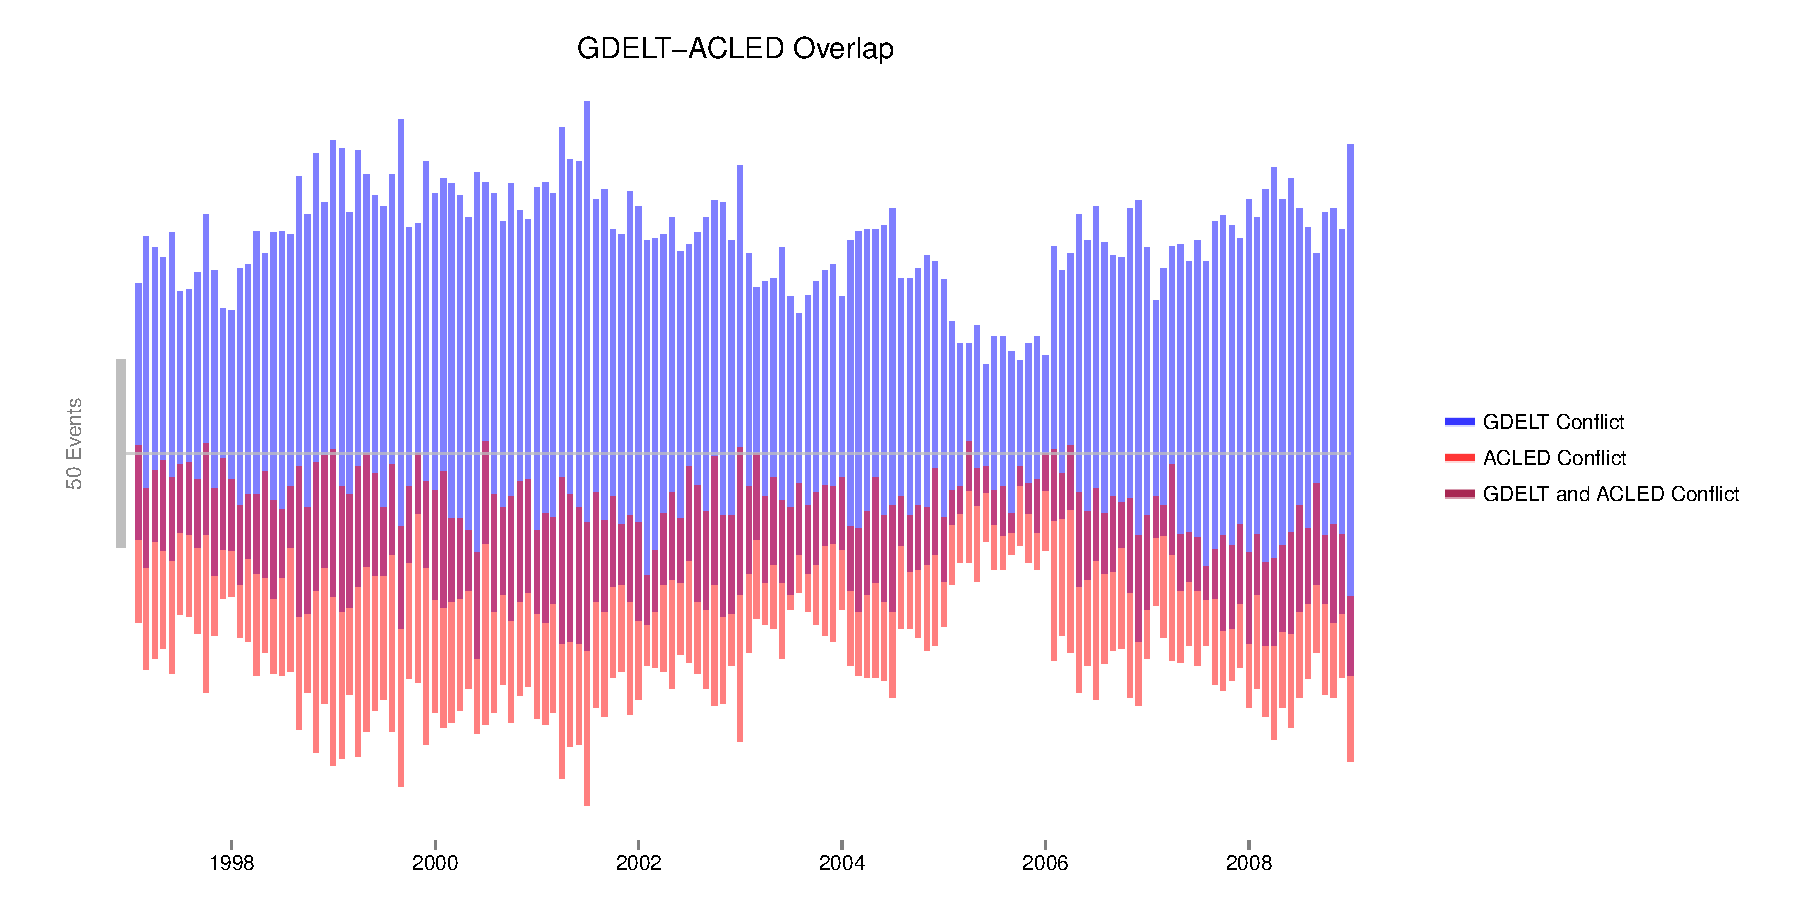
\includegraphics[width = 1 \textwidth]{timeACLEDa2.pdf}\\
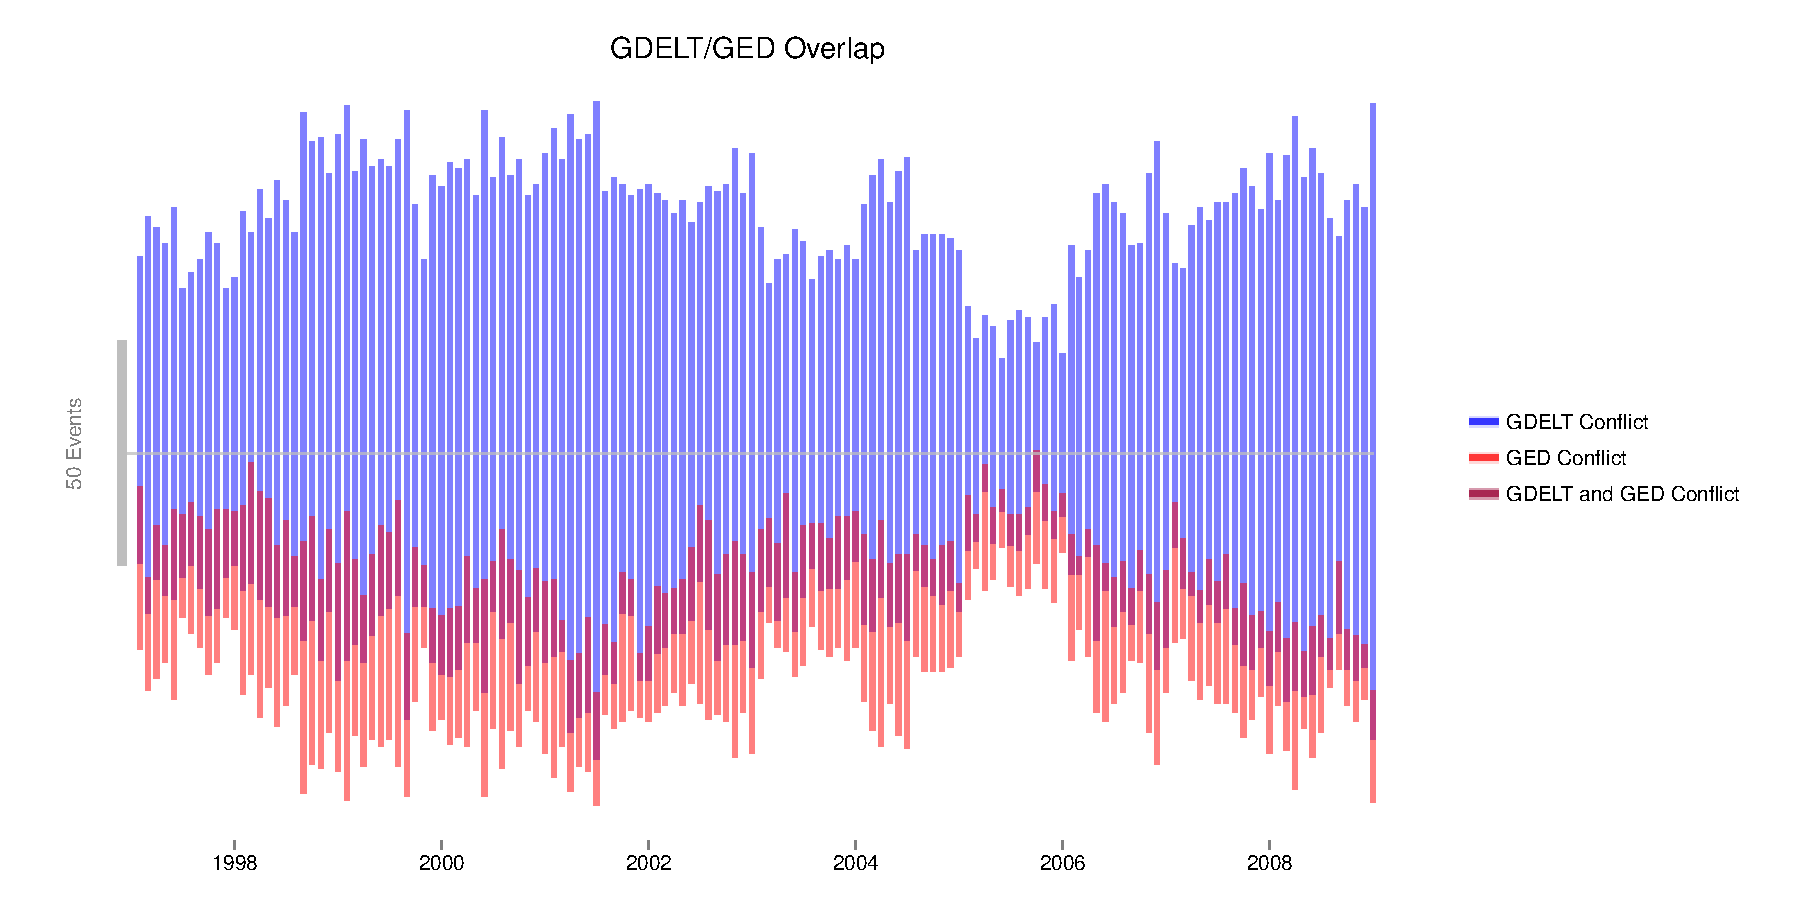
\includegraphics[width = 1 \textwidth]{timeGEDa2.pdf}
\caption{Grid-cell events over time}\label{fig:correlations_time}
\end{figure}

\begin{figure}[!htbp]
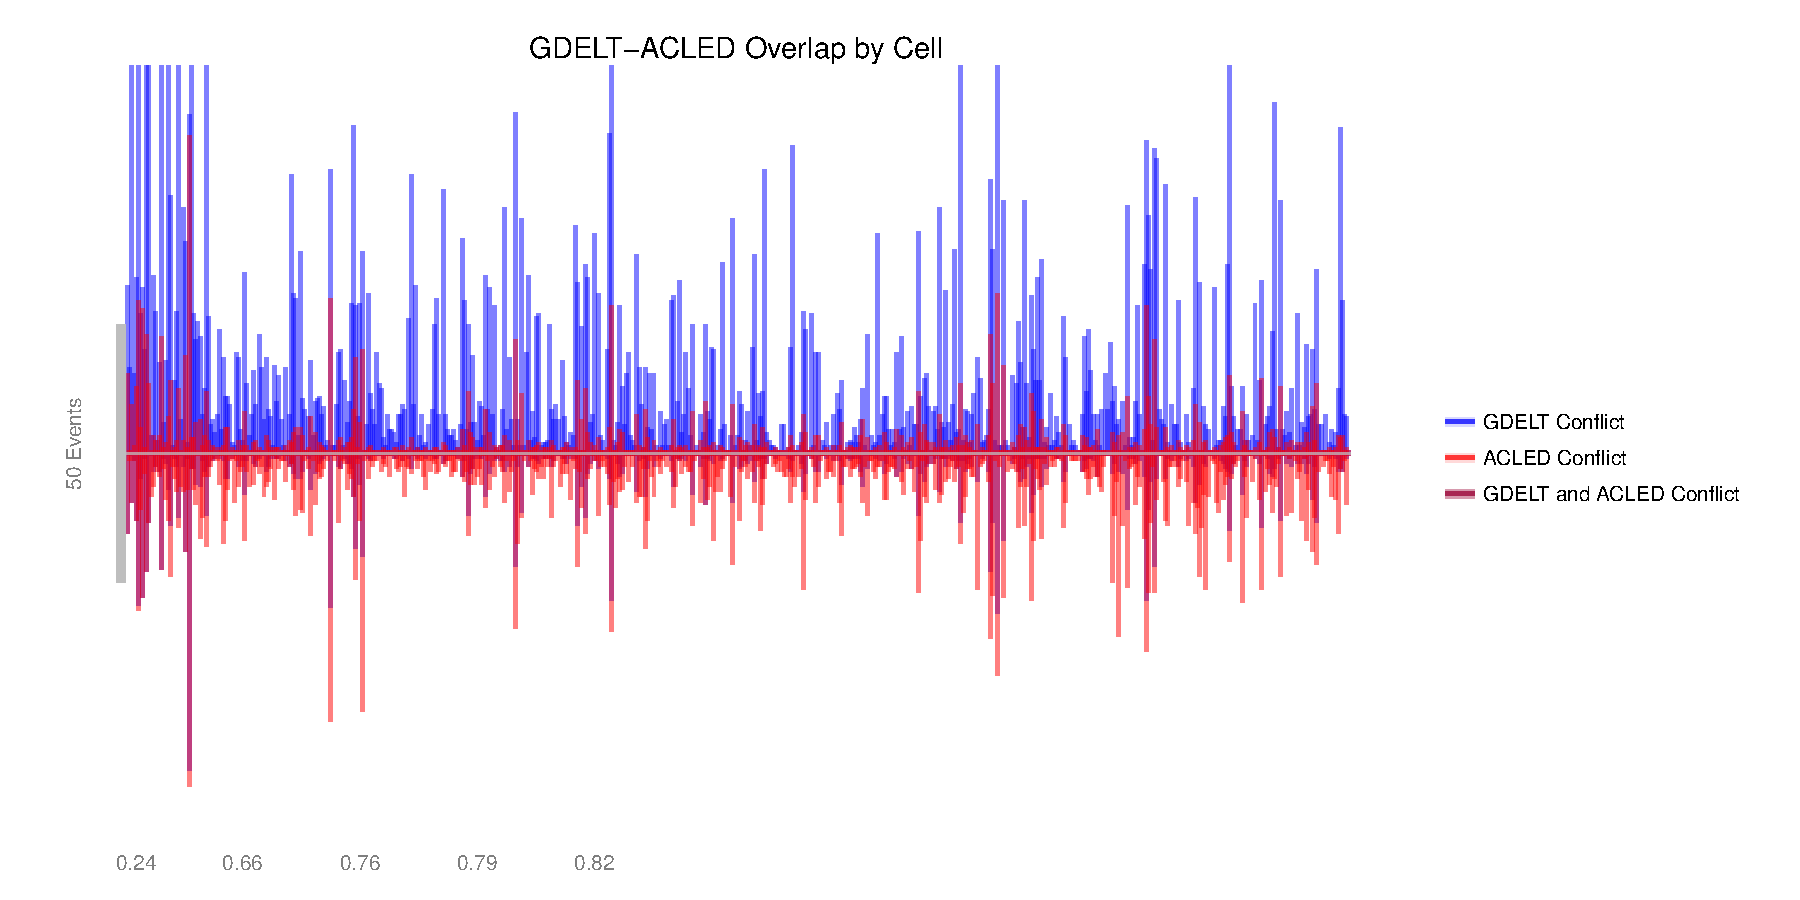
\includegraphics[width = 1 \textwidth]{spaceACLEDa2.pdf}\\
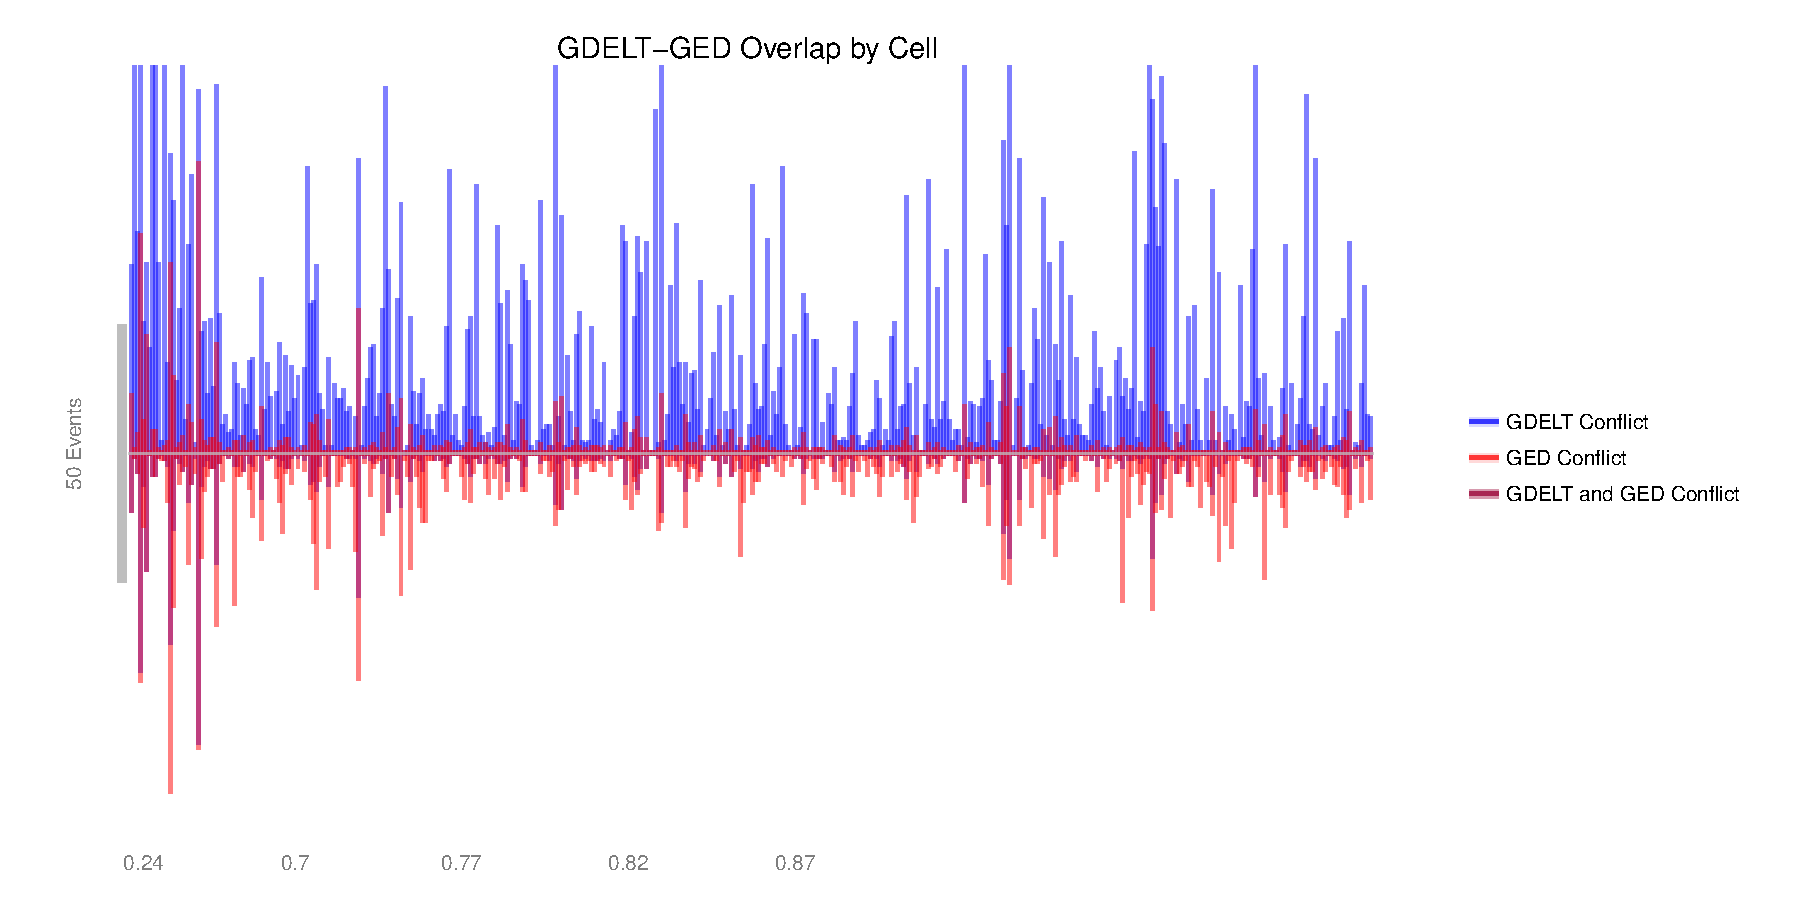
\includegraphics[width = 1 \textwidth]{spaceGEDa2.pdf}
\caption{Grid-cell events over logged and normalized capital distance}\label{fig:correlations_space}
\end{figure}
\newpage

% Table created by stargazer v.4.5.2 by Marek Hlavac, Harvard University. E-mail: hlavac at fas.harvard.edu
% Date and time: Thu, Dec 26, 2013 - 16:18:54
\begin{table}[!htbp] \centering 
  \caption{} 
  \label{} 
\begin{tabular}{@{\extracolsep{5pt}}lcccc} 
\\[-1.8ex]\hline 
\hline \\[-1.8ex] 
 & \multicolumn{4}{c}{\textit{Dependent variable:}} \\ 
\cline{2-5} 
\\[-1.8ex] & GDELT = 1, & GDELT = 0, & GDELT = 1, & GDELT = 0 \\ 
\\[-2.8ex] & ACLED = 0 & ACLED = 1 & GED = 0 & GED = 1 \\ 
\hline \\[-1.8ex] 
Population & 8.39$^{***}$ & 7.55$^{***}$ & 8.43$^{***}$ & 8.44$^{***}$ \\ 
  & (0.13) & (0.19) & (0.13) & (0.21) \\ 
  & & & & \\ 
Distance to Capital & $-$3.54$^{***}$ & 4.60$^{***}$ & $-$3.76$^{***}$ & 7.13$^{***}$ \\ 
  & (0.19) & (0.40) & (0.18) & (0.54) \\ 
  & & & & \\ 
 Constant & $-$20.82$^{***}$ & $-$27.49$^{***}$ & $-$20.52$^{***}$ & $-$33.45$^{***}$ \\ 
  & (0.51) & (0.89) & (0.49) & (1.34) \\ 
  & & & & \\ 
\hline \\[-1.8ex] 
Observations & 547,812 & 547,812 & 547,812 & 547,812 \\ 
\hline 
\hline \\[-1.8ex] 
\textit{Note:}  & \multicolumn{4}{r}{$^{*}$p$<$0.1; $^{**}$p$<$0.05; $^{***}$p$<$0.01} \\ 
\normalsize 
\end{tabular} 
\caption{Logit results: event mismatch by cell-month}
\end{table} 

\vfill

\newpage
% Table created by stargazer v.4.5.2 by Marek Hlavac, Harvard University. E-mail: hlavac at fas.harvard.edu
% Date and time: Thu, Dec 26, 2013 - 16:21:17
\begin{table}[!htbp] \centering 
  \caption{} 
  \label{} 
\begin{tabular}{@{\extracolsep{5pt}}lcccccc} 
\\[-1.8ex]\hline 
\hline \\[-1.8ex] 
 & \multicolumn{6}{c}{\textit{Dependent variable:}} \\ 
\cline{2-7} 
\\[-1.8ex] & \multicolumn{3}{c}{acled\_bin} & \multicolumn{3}{c}{ged\_bin} \\ 
\\[-1.8ex] & (1) & (2) & (3) & (4) & (5) & (6)\\ 
\hline \\[-1.8ex] 
ACLED (t-1) & 2.59$^{***}$ &  & 2.16$^{***}$ &  &  &  \\ 
  & (0.04) &  & (0.04) &  &  &  \\ 
  & & & & & & \\ 
ACLED spatial lag (t-1) & 0.06$^{***}$ &  & 0.06$^{***}$ &  &  &  \\ 
  & (0.003) &  & (0.003) &  &  &  \\ 
  & & & & & & \\ 
GDELT (t-1) &  & 1.91$^{***}$ & 1.30$^{***}$ &  & 1.80$^{***}$ & 1.26$^{***}$ \\ 
  &  & (0.03) & (0.04) &  & (0.04) & (0.05) \\ 
  & & & & & & \\ 
GDELT spatial lag (t-1) &  & 0.005$^{***}$ & $-$0.0002 &  & 0.004$^{***}$ & $-$0.004$^{***}$ \\ 
  &  & (0.0004) & (0.001) &  & (0.001) & (0.001) \\ 
  & & & & & & \\ 
GED (t-1) &  &  &  & 2.64$^{***}$ &  & 2.24$^{***}$ \\ 
  &  &  &  & (0.05) &  & (0.05) \\ 
  & & & & & & \\ 
GED spatial lag (t-1) &  &  &  & 0.13$^{***}$ &  & 0.14$^{***}$ \\ 
  &  &  &  & (0.01) &  & (0.01) \\ 
  & & & & & & \\ 
Distance to Capital & $-$0.16 & 1.24$^{***}$ & 1.04$^{***}$ & 1.34$^{***}$ & 1.82$^{***}$ & 2.38$^{***}$ \\ 
  & (0.25) & (0.23) & (0.25) & (0.31) & (0.28) & (0.31) \\ 
  & & & & & & \\ 
Population & 7.14$^{***}$ & 7.09$^{***}$ & 6.59$^{***}$ & 7.71$^{***}$ & 7.74$^{***}$ & 7.22$^{***}$ \\ 
  & (0.16) & (0.15) & (0.16) & (0.18) & (0.17) & (0.18) \\ 
  & & & & & & \\ 
 Constant & $-$21.28$^{***}$ & $-$22.21$^{***}$ & $-$21.25$^{***}$ & $-$24.28$^{***}$ & $-$24.79$^{***}$ & $-$24.34$^{***}$ \\ 
  & (0.61) & (0.58) & (0.61) & (0.71) & (0.67) & (0.71) \\ 
  & & & & & & \\ 
\hline \\[-1.8ex] 
Observations & 547,812 & 547,812 & 547,812 & 547,812 & 547,812 & 547,812 \\ 
Log Likelihood & $-$25,369.56 & $-$26,559.26 & $-$24,834.97 & $-$19,044.87 & $-$19,904.60 & $-$18,696.78 \\ 
Akaike Inf. Crit. & 50,797.11 & 53,176.52 & 49,731.95 & 38,147.73 & 39,867.20 & 37,455.57 \\ 
AUC & 0.89 & 0.88 & 0.89 & 0.87 & 0.86 & 0.88\\
\hline 
\hline \\[-1.8ex] 
\textit{Note:}  & \multicolumn{6}{r}{$^{*}$p$<$0.1; $^{**}$p$<$0.05; $^{***}$p$<$0.01} \\ 
\normalsize 
\end{tabular} 
\caption{Logit results: predicting conflict events}
\end{table}

\newpage
\subsection{Results using coding scheme 3 (high information requirements)}
High information requirements dramatically lower the number of `valid' GDELT observations. While all regression results hold substantively, the balance of false positives and false negatives shifts significantly.
% latex table generated in R 3.0.2 by xtable 1.7-1 package
% Thu Dec 26 17:24:40 2013
\begin{table}[ht]
\centering
\begin{tabular}{rrrr}
  \hline
 & ACLED & GED & GDELT \\ 
  \hline
ACLED & 1.00 & 0.32 & 0.21 \\ 
  GED & 0.32 & 1.00 & 0.15 \\ 
GDELT & 0.21 & 0.15 & 1.00 \\ 
   \hline
\end{tabular}
\caption{Correlations: Events by Cell-Month} 
\end{table}

% latex table generated in R 3.0.2 by xtable 1.7-1 package
% Thu Dec 26 17:25:00 2013
\begin{table}[ht]
\centering
\begin{tabular}{rrrr}
  \hline
 &  \multicolumn{3}{c}{ACLED}\\
 & 0 & 1 \\ 
  \hline
 GDELT & 0 & 540305 & 5908 \\ 
&  1 & 905 & 694 \\ 
   \hline
\end{tabular}
\caption{Confusion Matrix: ACLED} 
\end{table}

% latex table generated in R 3.0.2 by xtable 1.7-1 package
% Thu Dec 26 17:25:00 2013
\begin{table}[ht]
\centering
\begin{tabular}{rrrr}
  \hline
   &  \multicolumn{3}{c}{GED}\\
 & 0 & 1 \\ 
  \hline
GDELT & 0 & 542220 & 3993 \\ 
&  1 & 1180 & 419 \\ 
   \hline
\end{tabular}
\caption{Confusion Matrix: GED} 
\end{table}

\newpage
\begin{figure}[!htbp]
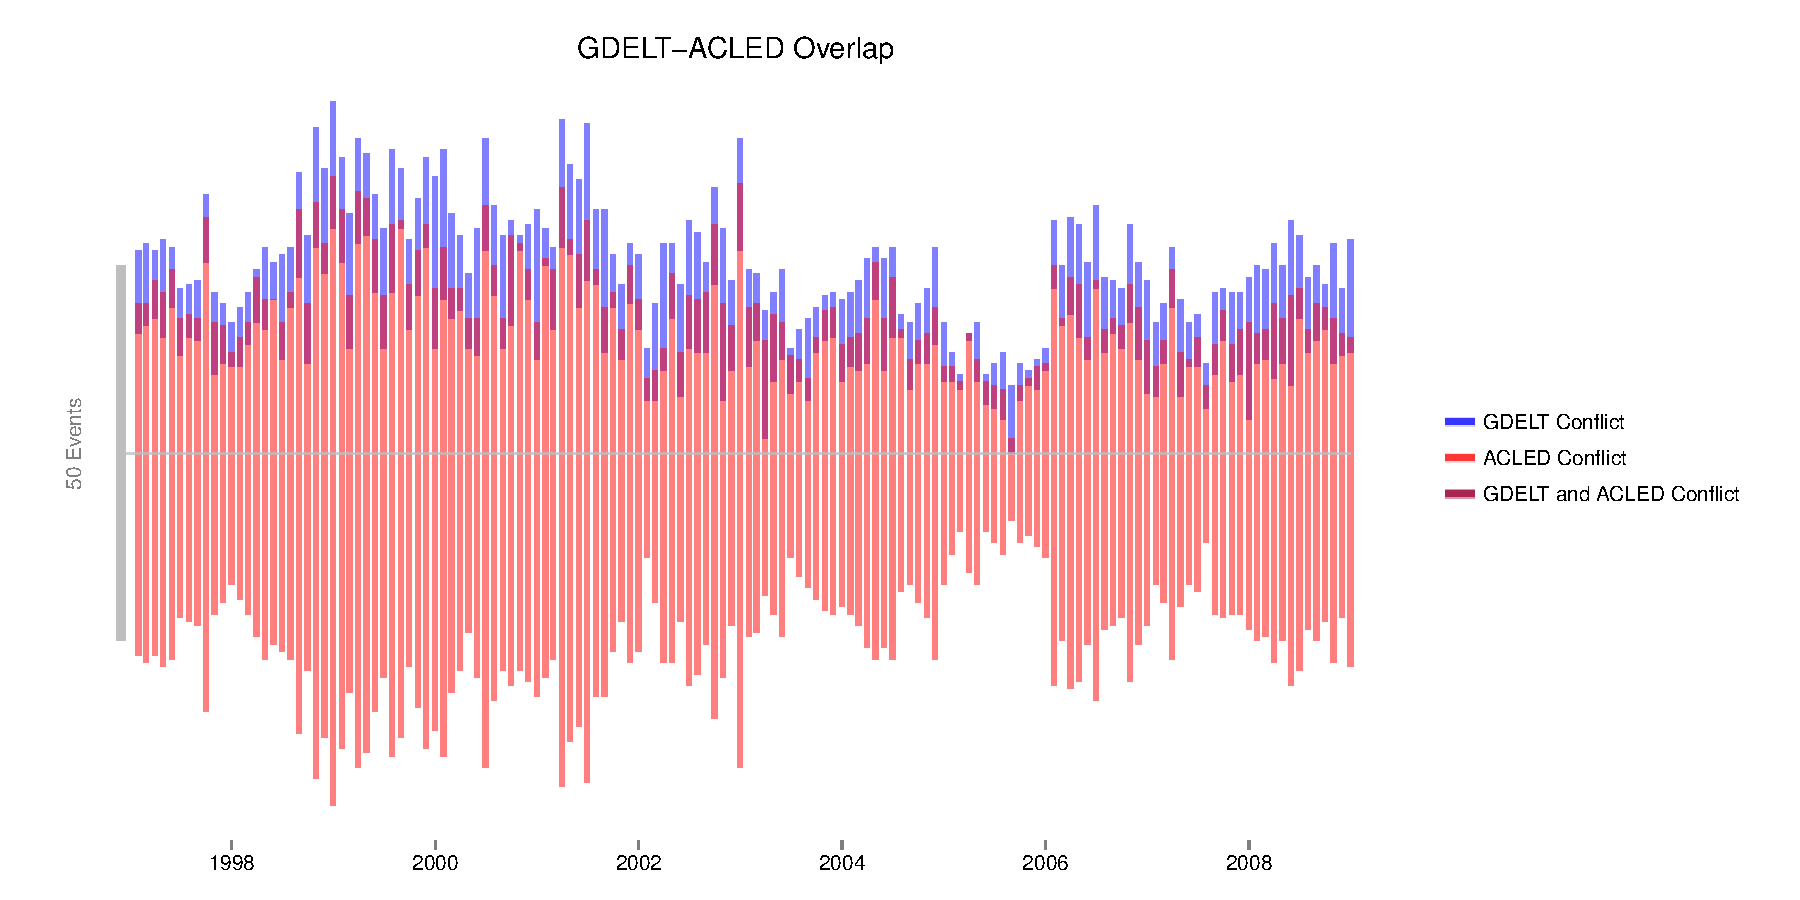
\includegraphics[width = 1 \textwidth]{timeACLEDa3.pdf}\\
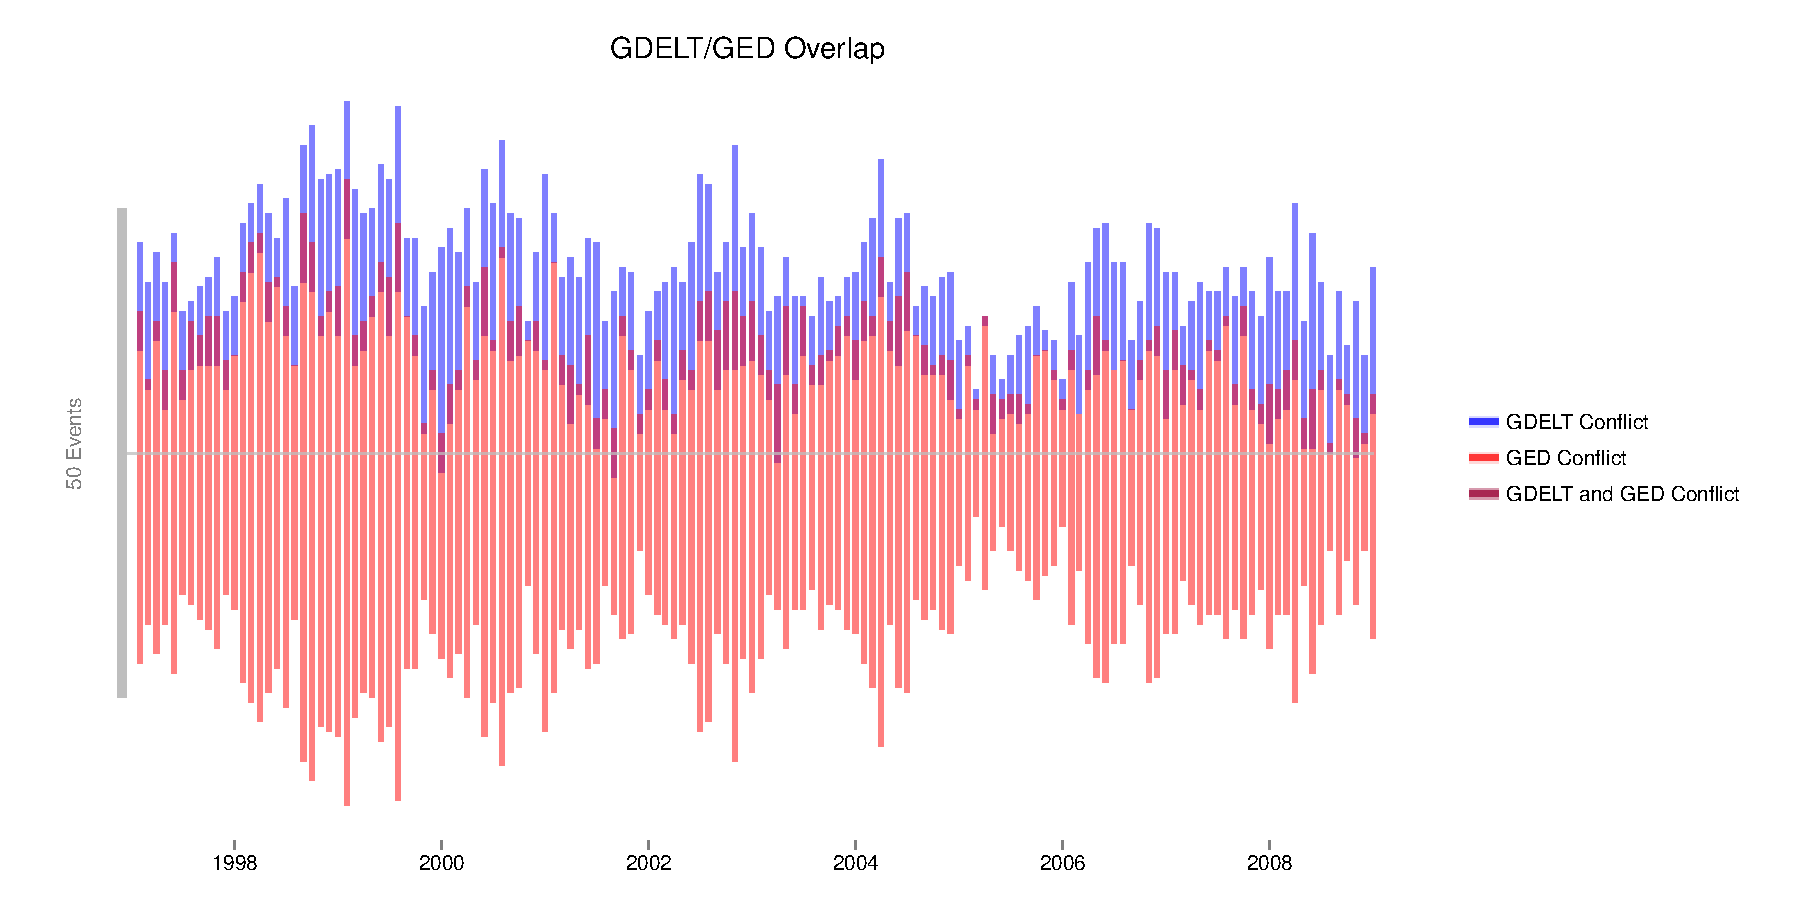
\includegraphics[width = 1 \textwidth]{timeGEDa3.pdf}
\caption{Grid-cell events over time}\label{fig:correlations_time}
\end{figure}

\begin{figure}[!htbp]
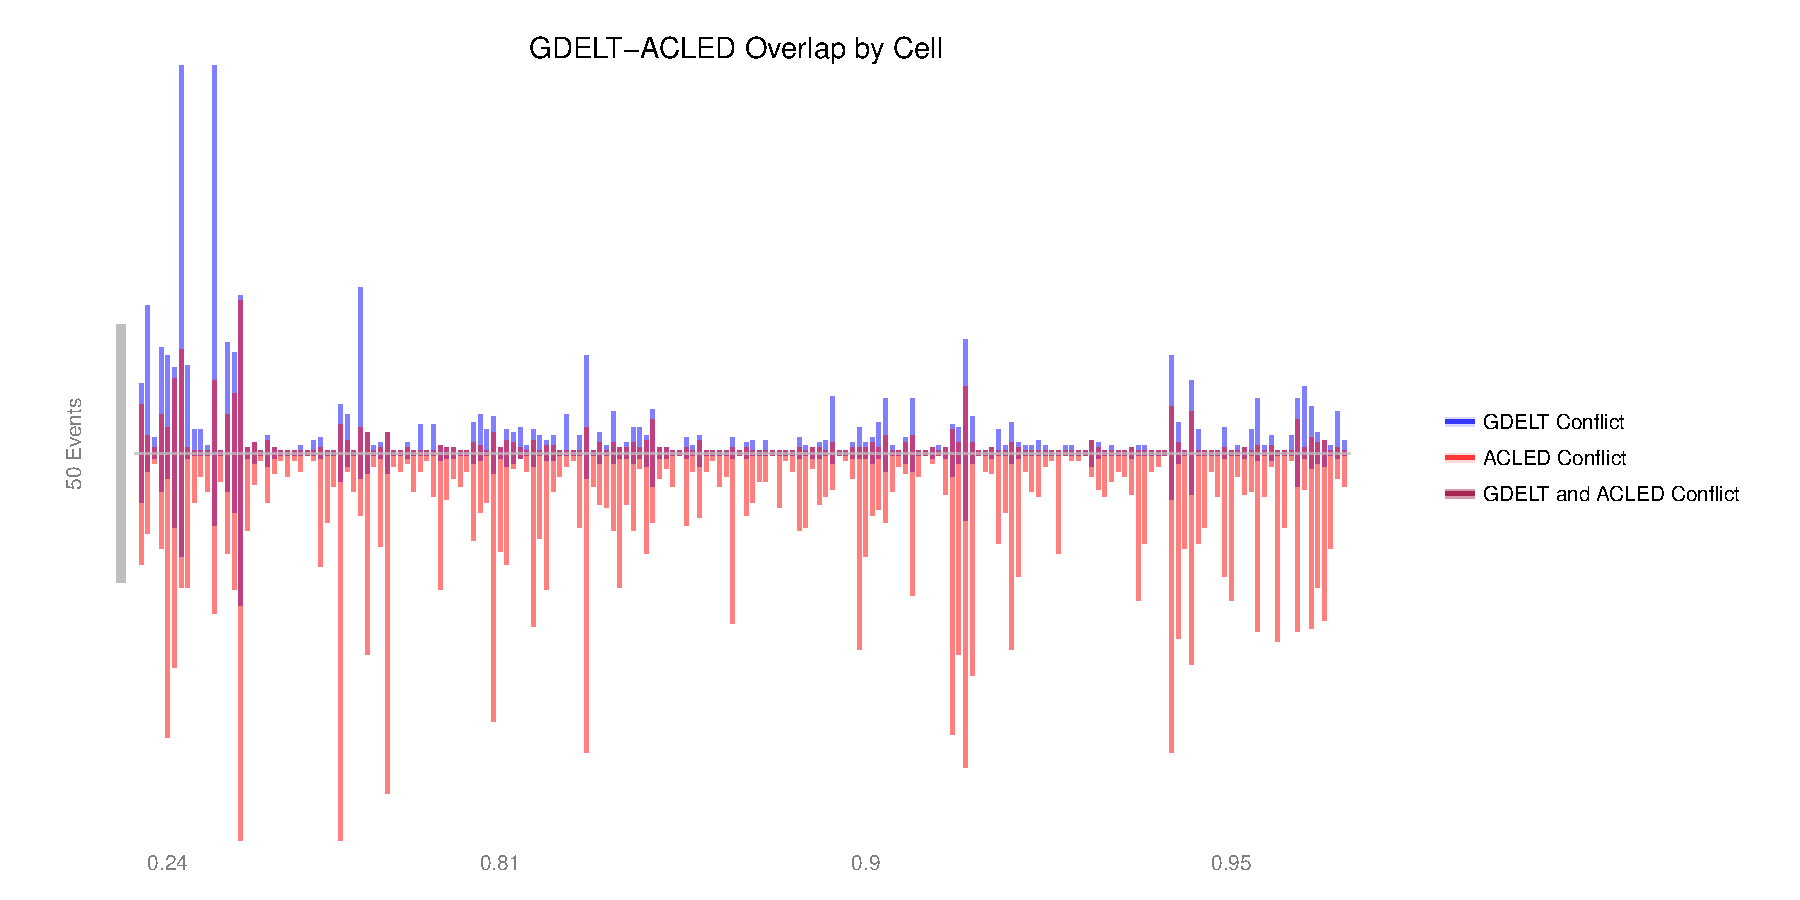
\includegraphics[width = 1 \textwidth]{spaceACLEDa3.pdf}\\
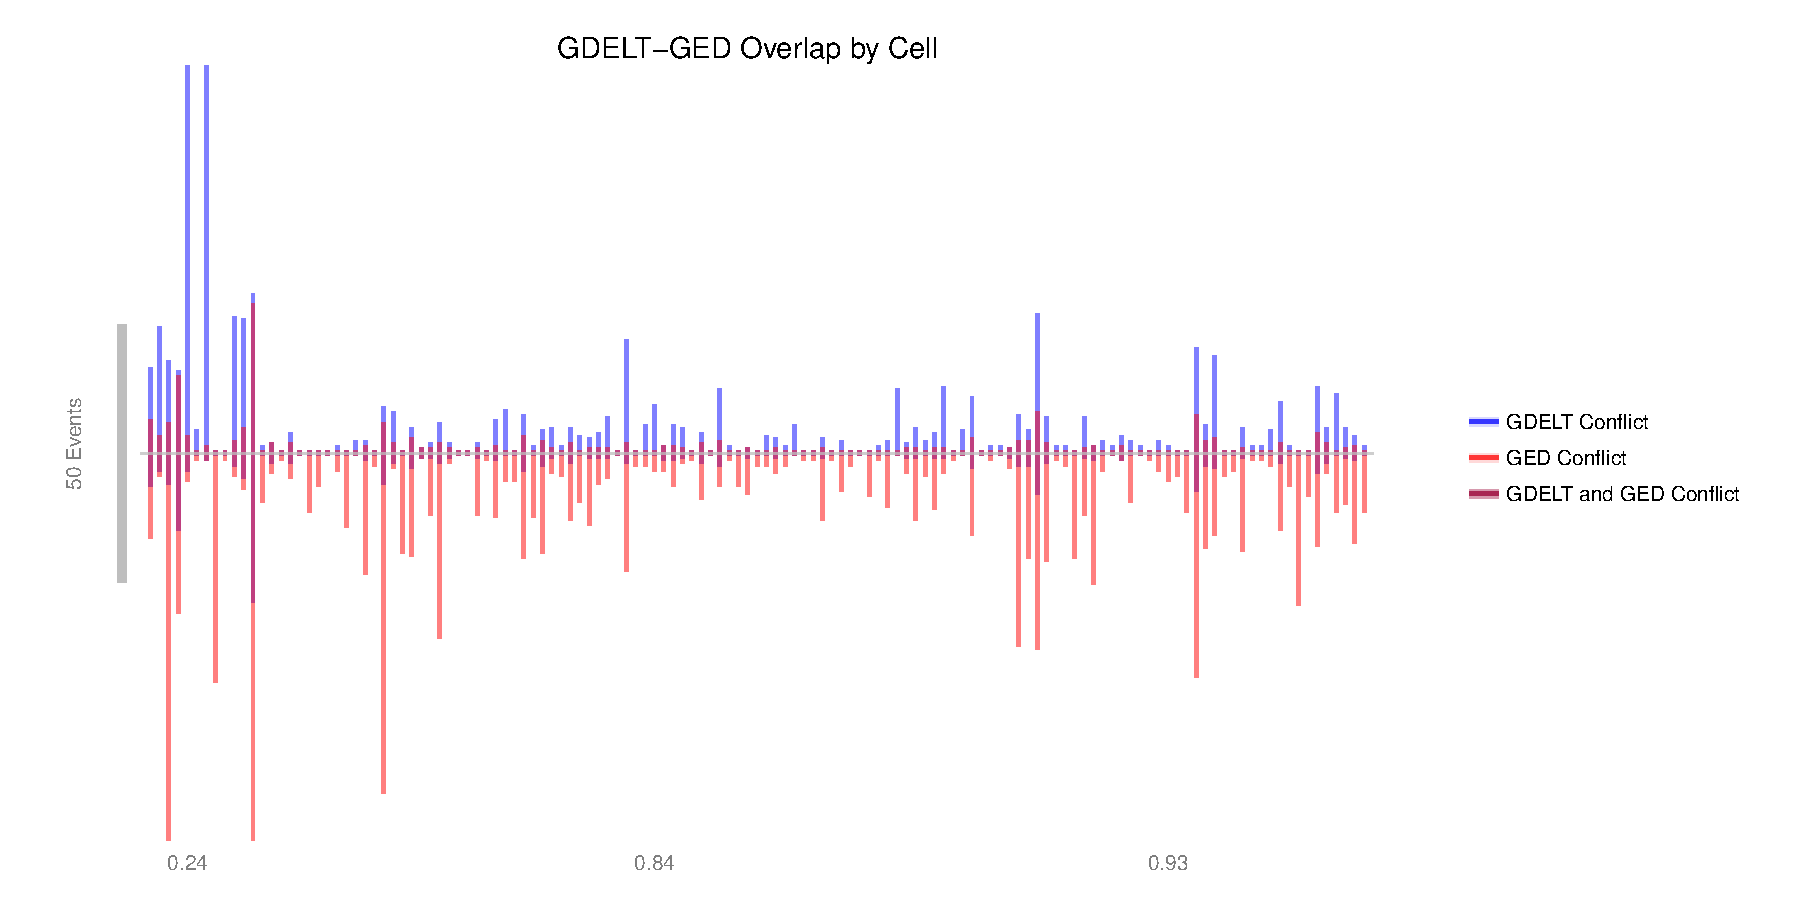
\includegraphics[width = 1 \textwidth]{spaceGEDa3.pdf}
\caption{Grid-cell events over logged and normalized capital distance}\label{fig:correlations_space}
\end{figure}
\newpage

% Table created by stargazer v.4.5.2 by Marek Hlavac, Harvard University. E-mail: hlavac at fas.harvard.edu
% Date and time: Thu, Dec 26, 2013 - 16:18:54
\begin{table}[!htbp] \centering 
  \caption{} 
  \label{} 
\begin{tabular}{@{\extracolsep{5pt}}lcccc} 
\\[-1.8ex]\hline 
\hline \\[-1.8ex] 
 & \multicolumn{4}{c}{\textit{Dependent variable:}} \\ 
\cline{2-5} 
\\[-1.8ex] & GDELT = 1, & GDELT = 0, & GDELT = 1, & GDELT = 0 \\ 
\\[-2.8ex] & ACLED = 0 & ACLED = 1 & GED = 0 & GED = 1 \\ 
\hline \\[-1.8ex] 
Population & 0.66$^{***}$ & 0.72$^{***}$ & 0.73$^{***}$ & 0.78$^{***}$ \\ 
  & (0.04) & (0.01) & (0.03) & (0.01) \\ 
  & & & & \\ 
Distance to Capital & $-$4.80$^{***}$ & 0.98$^{***}$ & $-$4.76$^{***}$ & 1.17$^{***}$ \\ 
  & (0.29) & (0.15) & (0.25) & (0.18) \\ 
  & & & & \\ 
 Constant & $-$21.19 & $-$12.13$^{***}$ & $-$10.27$^{***}$ & $-$13.43$^{***}$ \\ 
  & (211.60) & (0.37) & (1.14) & (0.46) \\ 
  & & & & \\ 
\hline \\[-1.8ex] 
Observations & 547,812 & 547,812 & 547,812 & 547,812 \\ 
\hline 
\hline \\[-1.8ex] 
\textit{Note:}  & \multicolumn{4}{r}{$^{*}$p$<$0.1; $^{**}$p$<$0.05; $^{***}$p$<$0.01} \\ 
\normalsize 
\end{tabular} 
\caption{Logit results: event mismatch by cell-month}
\end{table} 

\newpage
% Table created by stargazer v.4.5.2 by Marek Hlavac, Harvard University. E-mail: hlavac at fas.harvard.edu
% Date and time: Thu, Dec 26, 2013 - 17:26:42
\begin{table}[!htbp] \centering 
  \caption{} 
  \label{} 
\begin{tabular}{@{\extracolsep{5pt}}lcccccc} 
\\[-1.8ex]\hline 
\hline \\[-1.8ex] 
 & \multicolumn{6}{c}{\textit{Dependent variable:}} \\ 
\cline{2-7} 
\\[-1.8ex] & \multicolumn{3}{c}{acled\_bin} & \multicolumn{3}{c}{ged\_bin} \\ 
\\[-1.8ex] & (1) & (2) & (3) & (4) & (5) & (6)\\ 
\hline \\[-1.8ex] 
ACLED (t-1) & 2.59$^{***}$ &  & 2.49$^{***}$ &  &  &  \\ 
  & (0.04) &  & (0.04) &  &  &  \\ 
  & & & & & & \\ 
ACLED spatial lag (t-1) & 0.06$^{***}$ &  & 0.06$^{***}$ &  &  &  \\ 
  & (0.003) &  & (0.003) &  &  &  \\ 
  & & & & & & \\ 
GDELT (t-1) &  & 2.01$^{***}$ & 1.20$^{***}$ &  & 1.48$^{***}$ & 0.88$^{***}$ \\ 
  &  & (0.07) & (0.08) &  & (0.08) & (0.09) \\ 
  & & & & & & \\ 
GDELT spatial lag (t-1) &  & 0.09$^{***}$ & $-$0.01 &  & 0.07$^{***}$ & $-$0.01 \\ 
  &  & (0.01) & (0.01) &  & (0.01) & (0.01) \\ 
  & & & & & & \\ 
GED (t-1) &  &  &  & 2.64$^{***}$ &  & 2.57$^{***}$ \\ 
  &  &  &  & (0.05) &  & (0.05) \\ 
  & & & & & & \\ 
GDELT spatial lag (t-1) &  &  &  & 0.13$^{***}$ &  & 0.13$^{***}$ \\ 
  &  &  &  & (0.01) &  & (0.01) \\ 
  & & & & & & \\ 
Distance to Capital & 0.43$^{***}$ & 0.83$^{***}$ & 0.78$^{***}$ & 1.37$^{***}$ & 1.03$^{***}$ & 1.64$^{***}$ \\ 
  & (0.14) & (0.14) & (0.15) & (0.18) & (0.17) & (0.18) \\ 
  & & & & & & \\ 
Population & 0.63$^{***}$ & 0.72$^{***}$ & 0.63$^{***}$ & 0.68$^{***}$ & 0.77$^{***}$ & 0.68$^{***}$ \\ 
  & (0.01) & (0.01) & (0.01) & (0.01) & (0.01) & (0.01) \\ 
  & & & & & & \\ 
 Constant & $-$10.98$^{***}$ & $-$11.74$^{***}$ & $-$11.31$^{***}$ & $-$12.56$^{***}$ & $-$12.88$^{***}$ & $-$12.89$^{***}$ \\ 
  & (0.36) & (0.34) & (0.37) & (0.42) & (0.40) & (0.43) \\ 
  & & & & & & \\ 
\hline \\[-1.8ex] 
Observations & 547,812 & 547,812 & 547,812 & 547,812 & 547,812 & 547,812 \\ 
Log Likelihood & $-$25,369.63 & $-$27,610.05 & $-$25,248.91 & $-$19,058.69 & $-$20,635.24 & $-$19,014.39 \\ 
Akaike Inf. Crit. & 50,797.26 & 55,278.11 & 50,559.82 & 38,175.38 & 41,328.48 & 38,090.78 \\ 
AUC & 0.89 & 0.86 & 0.89 & 0.87 & 0.84 & 0.87\\
\hline 
\hline \\[-1.8ex] 
\textit{Note:}  & \multicolumn{6}{r}{$^{*}$p$<$0.1; $^{**}$p$<$0.05; $^{***}$p$<$0.01} \\ 
\normalsize 
\end{tabular}
\caption{Logit results: predicting conflict events}
\end{table} 


\section*{Appendix C: Robustness Checks using Count Data}
The dependent variable in these models is therefore the number of events occurring in a given cell-month, not the general presence or absence of any violent events. In this case as well, the ability of GDELT to predict ACLED/GED events remains robust.

% latex table generated in R 3.0.2 by xtable 1.7-1 package
% Thu Dec 26 15:58:52 2013
\begin{table}[ht]
\centering
\begin{tabular}{rrrr}
  \hline
 & GDELT & ACLED & GED \\ 
  \hline
GDELT & 1.00 & 0.31 & 0.34 \\ 
  ACLED & 0.31 & 1.00 & 0.48 \\ 
GED & 0.34 & 0.48 & 1.00 \\ 
   \hline
\end{tabular}
\caption{Correlations: Number of Events by Cell-Month} 
\end{table}

% Table created by stargazer v.4.5.2 by Marek Hlavac, Harvard University. E-mail: hlavac at fas.harvard.edu
% Date and time: Thu, Dec 26, 2013 - 16:02:51
\begin{table}[!htbp] \centering 
  \caption{} 
  \label{} 
\begin{tabular}{@{\extracolsep{5pt}}lcccccc} 
\\[-1.8ex]\hline 
\hline \\[-1.8ex] 
 & \multicolumn{6}{c}{\textit{Dependent variable:}} \\ 
\cline{2-7} 
\\[-1.8ex] & \multicolumn{3}{c}{acled} & \multicolumn{3}{c}{ged} \\ 
\\[-1.8ex] & (1) & (2) & (3) & (4) & (5) & (6)\\ 
\hline \\[-1.8ex] 
ACLED (t-1) & 0.49$^{***}$ &  & 0.47$^{***}$ &  &  &  \\ 
  & (0.001) &  & (0.001) &  &  &  \\ 
  & & & & & & \\ 
ACLED spatial lag (t-1) & 0.01$^{***}$ &  & 0.02$^{***}$ &  &  &  \\ 
  & (0.0004) &  & (0.0004) &  &  &  \\ 
  & & & & & & \\ 
GDELT (t-1) &  & 0.19$^{***}$ & 0.07$^{***}$ &  & 0.12$^{***}$ & 0.05$^{***}$ \\ 
  &  & (0.001) & (0.001) &  & (0.001) & (0.001) \\ 
  & & & & & & \\ 
GDELT spatial lag (t-1) &  & 0.01$^{***}$ & $-$0.004$^{***}$ &  & 0.001$^{***}$ & $-$0.003$^{***}$ \\ 
  &  & (0.0004) & (0.0004) &  & (0.0002) & (0.0002) \\ 
  & & & & & & \\ 
GED (t-1) &  &  &  & 0.51$^{***}$ &  & 0.47$^{***}$ \\ 
  &  &  &  & (0.001) &  & (0.001) \\ 
  & & & & & & \\ 
GED spatial lag (t-1) &  &  &  & 0.01$^{***}$ &  & 0.02$^{***}$ \\ 
  &  &  &  & (0.0004) &  & (0.0004) \\ 
  & & & & & & \\ 
Distance to Capital & $-$0.09$^{***}$ & $-$0.04$^{***}$ & $-$0.06$^{***}$ & $-$0.06$^{***}$ & $-$0.06$^{***}$ & $-$0.05$^{***}$ \\ 
  & (0.01) & (0.01) & (0.01) & (0.004) & (0.005) & (0.004) \\ 
  & & & & & & \\ 
Population & 0.004$^{***}$ & 0.01$^{***}$ & 0.004$^{***}$ & 0.002$^{***}$ & 0.01$^{***}$ & 0.002$^{***}$ \\ 
  & (0.0004) & (0.0005) & (0.0004) & (0.0002) & (0.0002) & (0.0002) \\ 
  & & & & & & \\ 
 Constant & 0.14$^{***}$ & 0.17$^{***}$ & 0.11$^{***}$ & 0.05$^{***}$ & 0.04$^{***}$ & 0.04$^{***}$ \\ 
  & (0.02) & (0.03) & (0.02) & (0.01) & (0.01) & (0.01) \\ 
  & & & & & & \\ 
\hline \\[-1.8ex] 
Observations & 547,812 & 547,812 & 547,812 & 547,812 & 547,812 & 547,812 \\ 
Adjusted R$^{2}$ & 0.29 & 0.10 & 0.29 & 0.29 & 0.10 & 0.30 \\ 
\hline 
\hline \\[-1.8ex] 
\textit{Note:}  & \multicolumn{6}{r}{$^{*}$p$<$0.1; $^{**}$p$<$0.05; $^{***}$p$<$0.01} \\ 
\normalsize 
\end{tabular} 
\caption{Regression results: number of conflict events per cell-month}
\end{table} 


\pagebreak

\section*{Appendix D: Robustness Checks with Limited ACLED/GED Sources}
This section shows figures and tables summarizing results of parallel analysis using only a subset of ACLED and GED sources to match the sources used by GDELT as closely as possible: only event records derived from Associated Press, Agence France Presse, Xinhua News Service or BBC Monitoring were used.


\begin{table}[!htbp] \centering 
\begin{tabular}{@{\extracolsep{5pt}}lcc|cc} 
& \multicolumn{1}{c}{ACLED = 0} & \multicolumn{1}{c}{ACLED = 1} & \multicolumn{1}{c}{GED = 0} & \multicolumn{1}{c}{GED = 1} \\ 
\hline \\[-1.8ex] 
GDELT = 0 & 541,537 & 2,546  & 541,941 & 2,142\\ 
GDELT = 1 & 2,988 & 741  & 3,172 & 557 \\ 
\hline \\[-1.8ex] 
N = 547,812 Cell-Months\\
\normalsize 
\end{tabular} 
 \caption{Confusion Matrices, 4 major sources only.}\label{tab:confusion}
\end{table} 


\begin{figure}[!htbp]
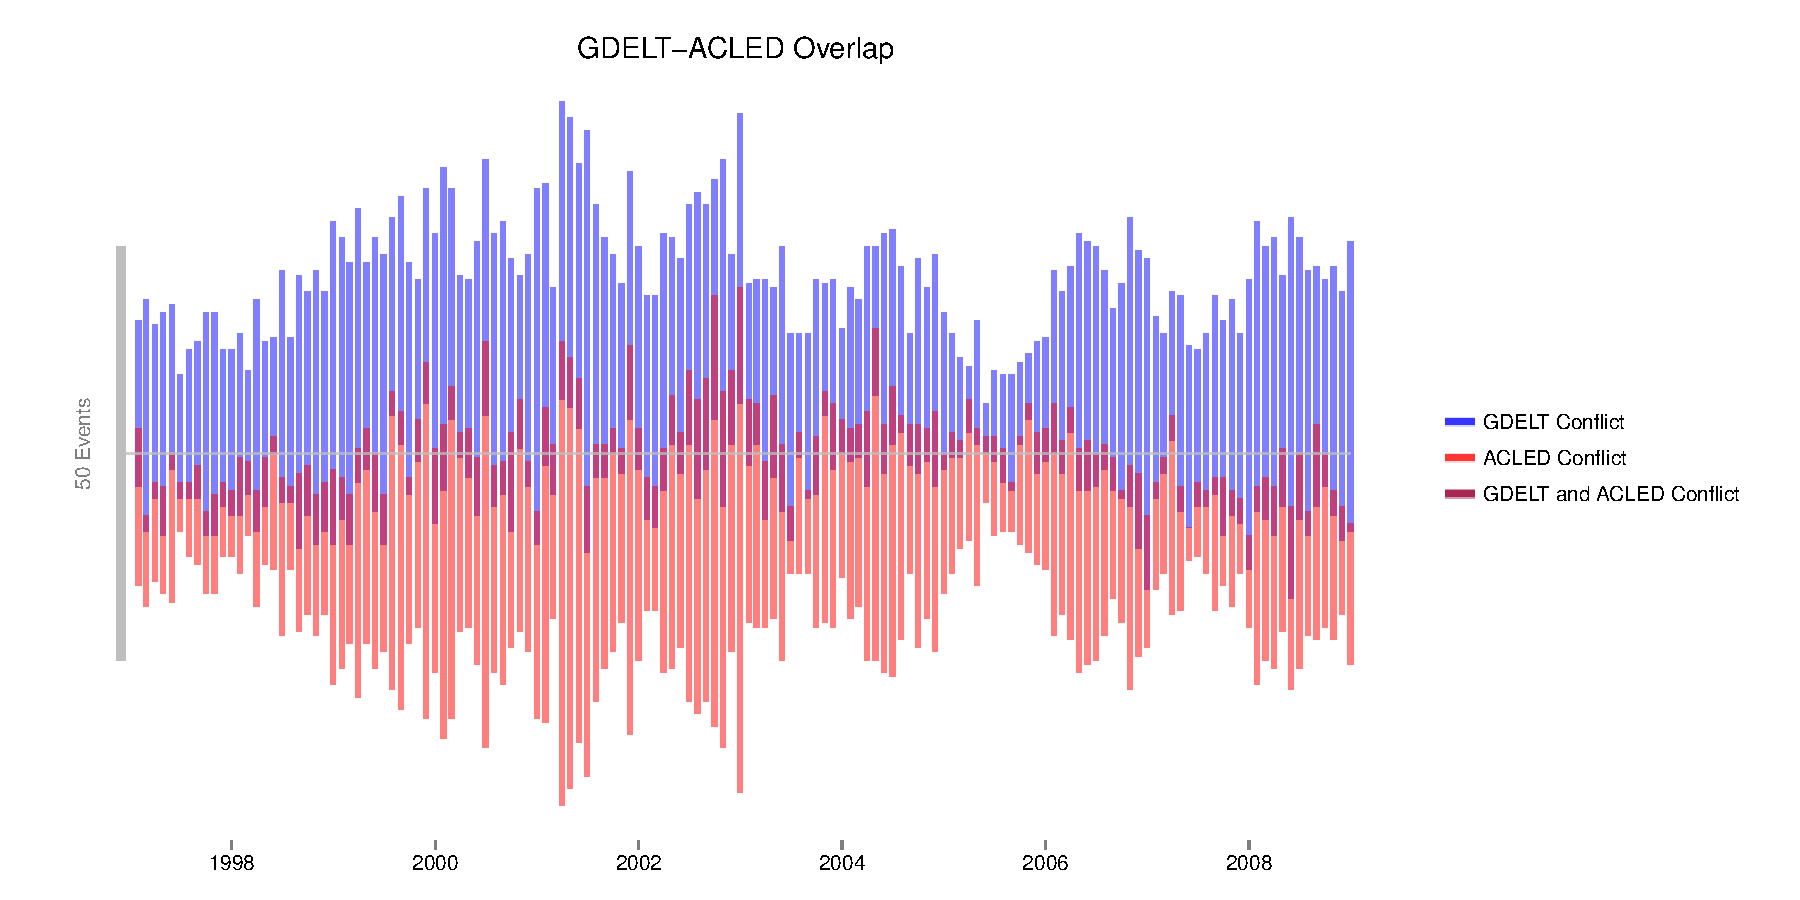
\includegraphics[width = 1 \textwidth]{timeACLED4source.pdf}\\
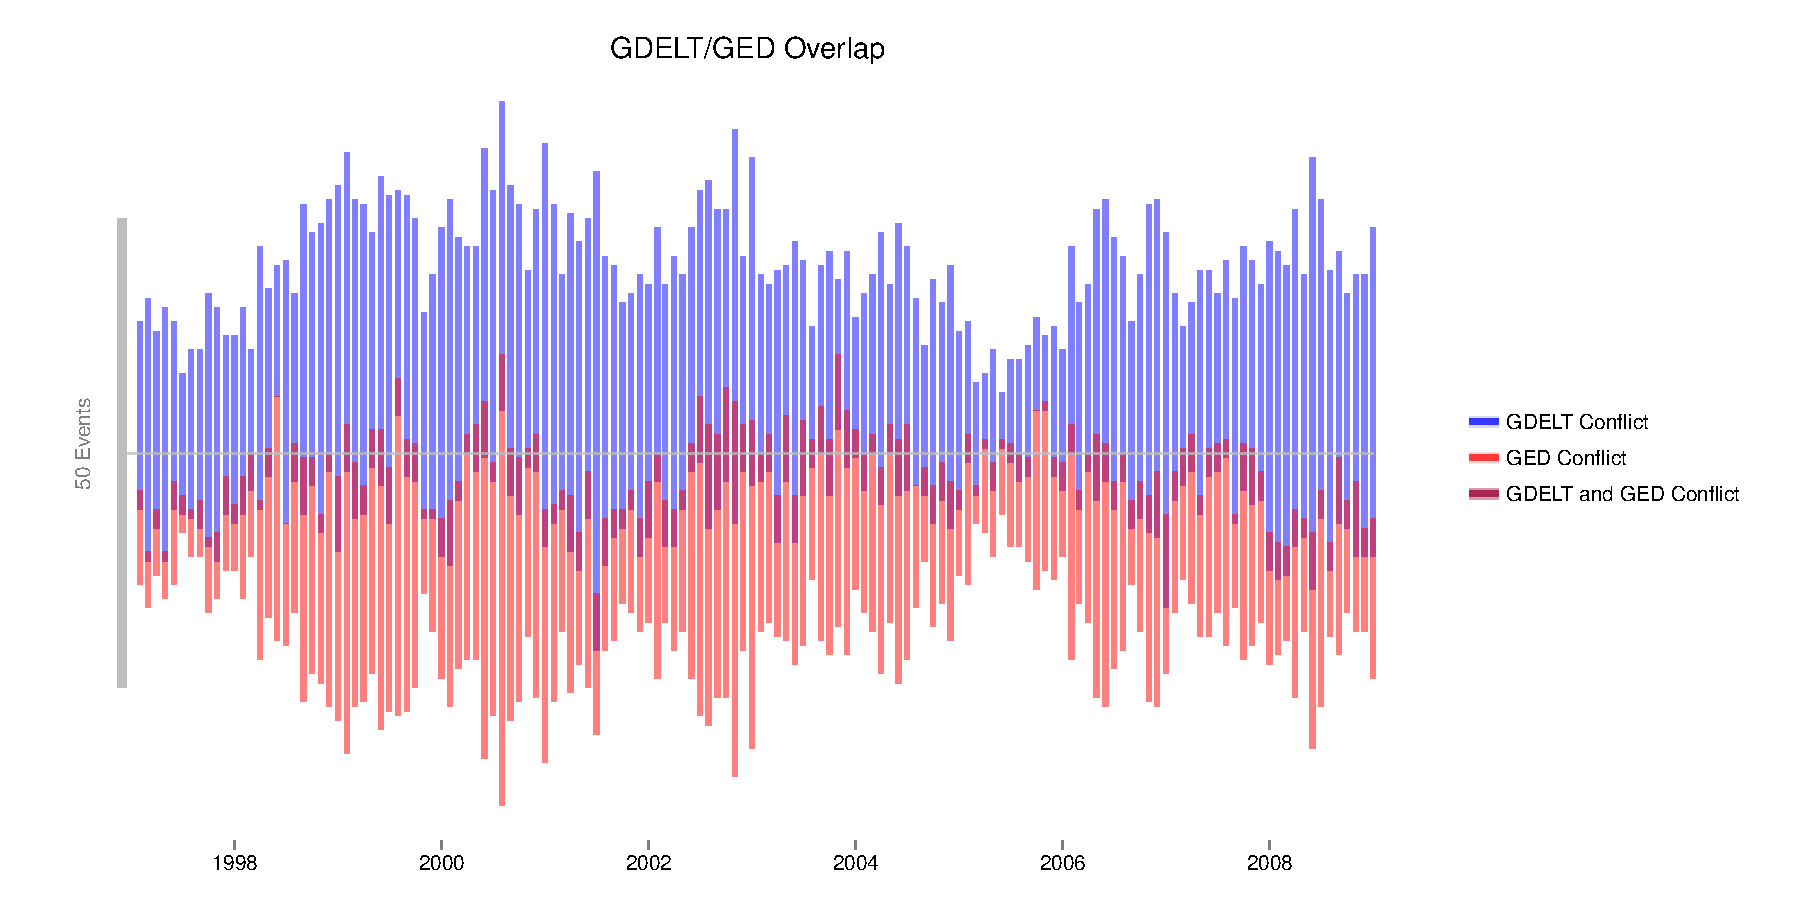
\includegraphics[width = 1 \textwidth]{timeGED4source.pdf}
\caption{Grid-cell events over time, 4 main sources only.}\label{fig:correlations_time}
\end{figure}

\begin{figure}[!htbp]
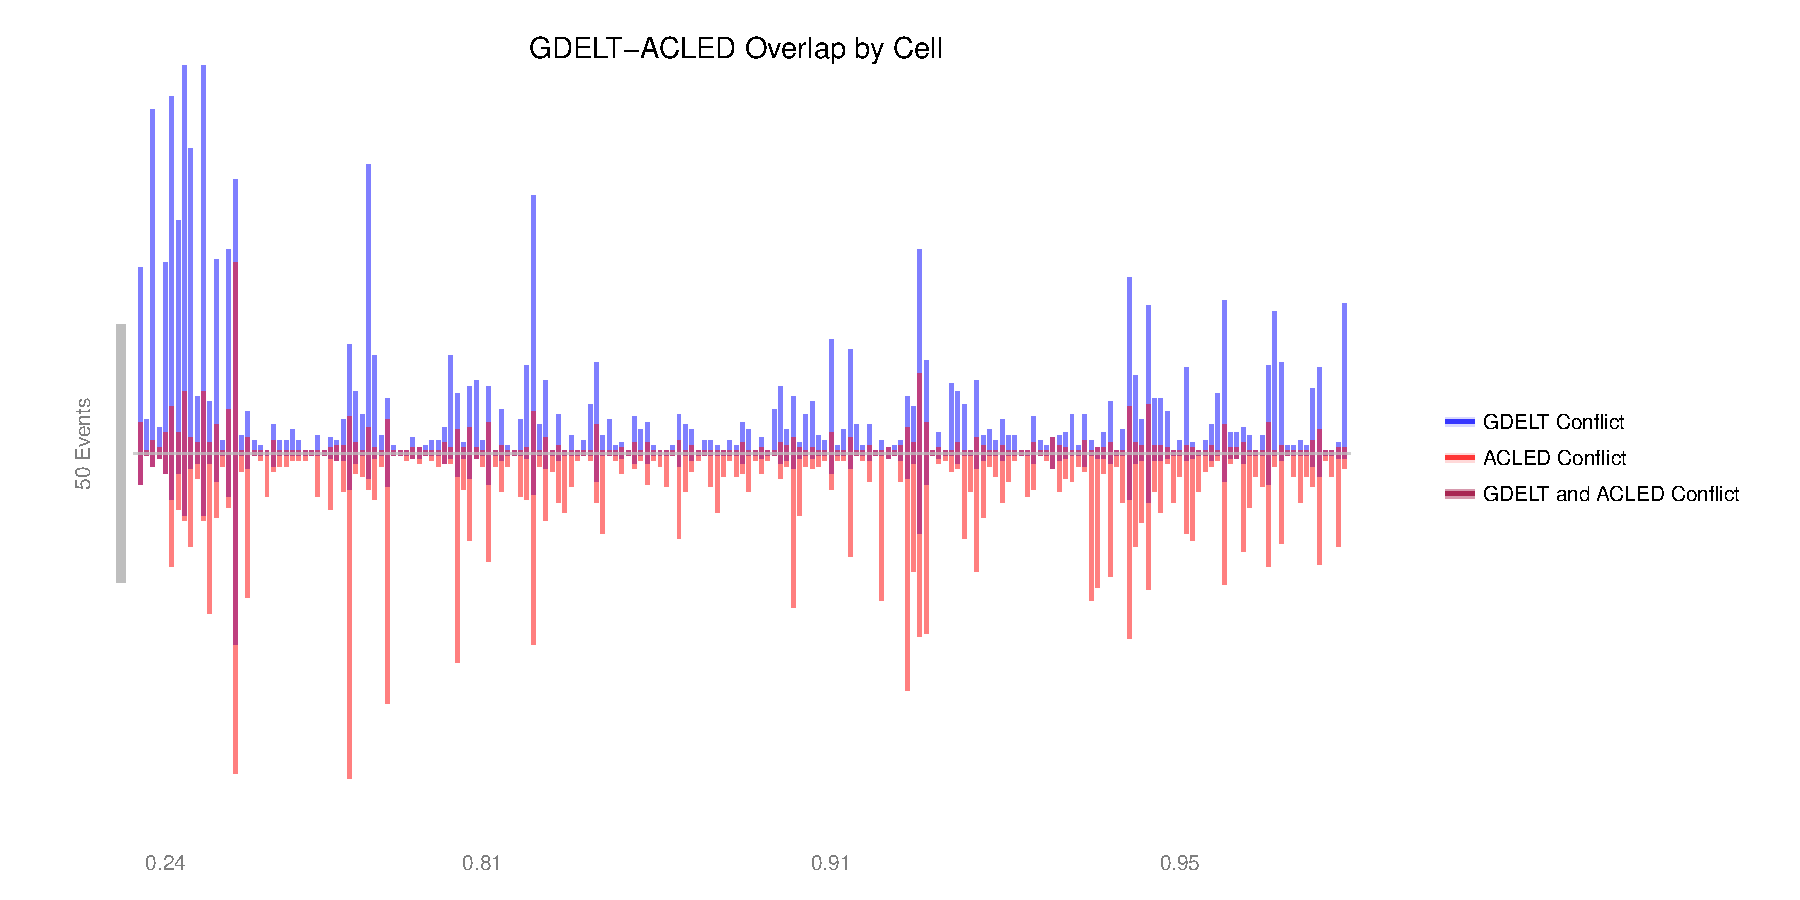
\includegraphics[width = 1 \textwidth]{spaceACLED4source.pdf}\\
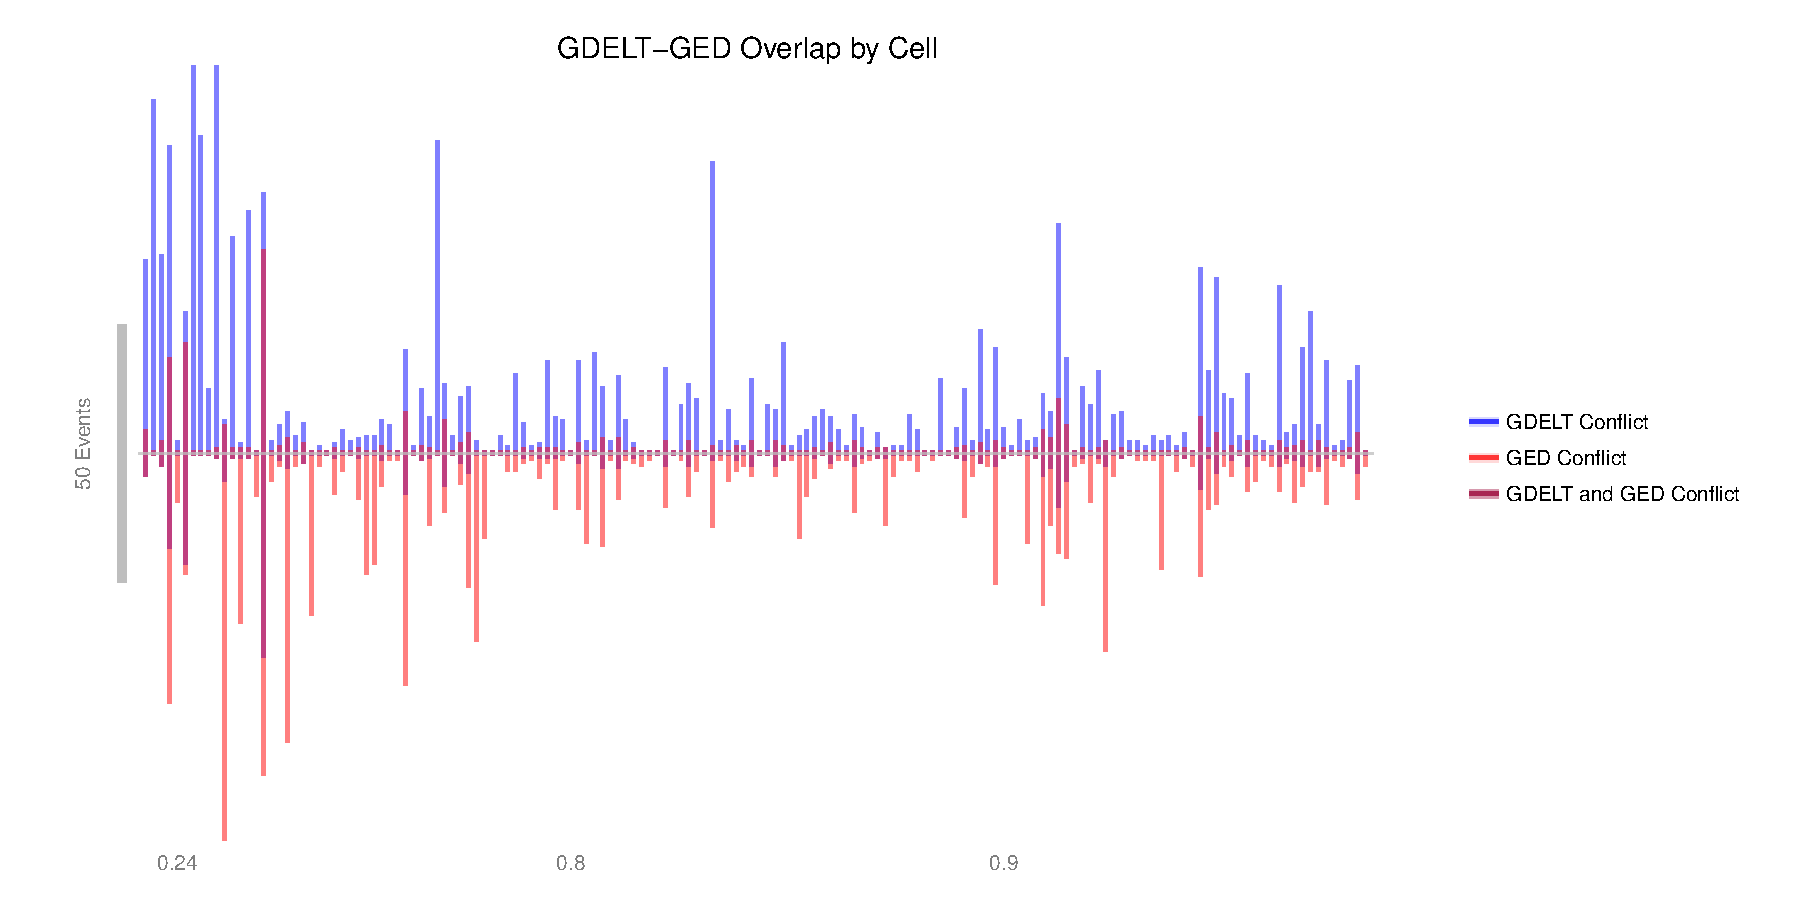
\includegraphics[width = 1 \textwidth]{spaceGED4source.pdf}
\caption{Grid-cell events over logged and normalized capital distance, 4 main sources only.}\label{fig:correlations_space}
\end{figure}



% Table created by stargazer v.4.5.2 by Marek Hlavac, Harvard University. E-mail: hlavac at fas.harvard.edu
% Date and time: Sat, Dec 21, 2013 - 11:43:23
\begin{table}[!htbp] \centering 
\begin{tabular}{@{\extracolsep{5pt}}lcccc} 
\\[-1.8ex]\hline 
\hline \\[-1.8ex] 
 & \multicolumn{2}{c}{\textit{GDELT-ACLED}} & \multicolumn{2}{c}{\textit{GDELT-GED}}\\ 
\cline{2-5} 
\\[-1.8ex] & GDELT = 1, & GDELT = 0, & GDELT = 1, & GDELT = 0 \\ 
\\[-2.8ex] & ACLED = 0 & ACLED = 1 & GED = 0 & GED = 1 \\ 
\\[-1.8ex] & (1) & (2) & (3) & (4)\\ 
\hline \\[-1.8ex] 
Population & 0.78$^{***}$ & 0.70$^{***}$ & 0.78$^{***}$ & 0.74$^{***}$ \\ 
  & (0.02) & (0.02) & (0.02) & (0.02) \\ 
  & & & & \\ 
 Distance to Capital & $-$3.53$^{***}$ & 2.49$^{***}$ & $-$3.36$^{***}$ & 0.27 \\ 
  & (0.17) & (0.24) & (0.17) & (0.25) \\ 
  & & & & \\ 
 Constant & $-$10.35$^{***}$ & $-$12.46$^{***}$ & $-$10.50$^{***}$ & $-$14.17$^{***}$ \\ 
  & (0.68) & (0.45) & (0.68) & (0.51) \\ 
    & & & & \\ 
\hline \\[-1.8ex] 
Observations & 547,812 & 547,812 & 547,812 & 547,812 \\ 
\hline 
\hline \\[-1.8ex] 
\textit{Note:}  & \multicolumn{4}{r}{$^{*}$p$<$0.1; $^{**}$p$<$0.05; $^{***}$p$<$0.01} \\ 
			& \multicolumn{4}{r}{Country-level fixed effects not shown.} \\ 
\normalsize 
\end{tabular} 
  \caption{Logistic regression results: event record disagreement by cell-month, 4 major sources only.}\label{tab:regression1}
\end{table} 




% Table created by stargazer v.4.5.2 by Marek Hlavac, Harvard University. E-mail: hlavac at fas.harvard.edu
% Date and time: Sat, Dec 21, 2013 - 10:34:33
\begin{table}[!htbp] \centering 
\begin{footnotesize}
  \begin{tabular}{@{\extracolsep{5pt}}lcccccc} 
\cline{2-7} 
\\[-1.8ex] & \multicolumn{3}{c}{ACLED Conflict} & \multicolumn{3}{c}{GED Conflict} \\ 
\\[-1.8ex] & (1) & (2) & (3) & (4) & (5) & (6)\\ 
\hline \\[-1.8ex] 
 Conflict (t-1) & 2.63$^{***}$ &  & 2.41$^{***}$ & 2.64$^{***}$ &  & 2.49$^{***}$ \\ 
  & (0.05) &  & (0.06) & (0.06) &  & (0.06) \\ 
  & & & & & & \\ 
 Spatial lag (t-1) & 0.10$^{***}$ &  & 0.09$^{***}$& 0.16$^{***}$ &  & 0.18$^{***}$ \\ 
  & (0.01) &  & (0.01) & (0.01) &  & (0.01) \\ 
  & & & & & & \\ 
  GDELT conflict (t-1) &  & 1.75$^{***}$ & 1.19$^{***}$ &  & 1.46$^{***}$ & 0.99$^{***}$ \\ 
  &  & (0.06) & (0.07) &  & (0.07) & (0.08) \\ 
  & & & & & & \\ 
 GDELT spatial lag (t-1) &  & 0.03$^{***}$ & 0.01 &  & 0.02$^{***}$ & $-$0.01$^{*}$ \\ 
  &  & (0.004) & (0.01) &  & (0.004) & (0.01) \\ 
  & & & & & & \\ 
  Distance to Capital & 0.81$^{***}$ & 1.75$^{***}$ & 1.47$^{***}$ & 0.28 & 0.13 & 0.83$^{***}$ \\ 
  & (0.20) & (0.20) & (0.21) & (0.23) & (0.21) & (0.23) \\ 
  & & & & & & \\ 
  Population & 0.65$^{***}$ & 0.68$^{***}$ & 0.63$^{***}$ & 0.66$^{***}$ & 0.73$^{***}$ & 0.66$^{***}$ \\ 
  & (0.02) & (0.02) & (0.02) & (0.02) & (0.02) & (0.02) \\ 
  & & & & & & \\ 
 Constant & $-$11.99$^{***}$ & $-$13.14$^{***}$ & $-$12.48$^{***}$ & $-$11.98$^{***}$ & $-$12.48$^{***}$ & $-$12.57$^{***}$ \\ 
  & (0.51) & (0.50) & (0.51) & (0.56) & (0.54) & (0.57) \\ 
  & & & & & & \\ 
\hline \\[-1.8ex] 
Observations & 547,812 & 547,812 & 547,812 & 547,812 & 547,812 & 547,812 \\ 
Log Likelihood & $-$14,267.93 & $-$15,171.26 & $-$14,131.63 & $-$12,190.99 & $-$13,031.73 & $-$12,117.83 \\ 
Akaike Inf. Crit. & 28,593.87 & 30,400.52 & 28,325.26 & 24,439.98 & 26,121.47 & 24,297.66 \\ 
AUC 		& 0.90 & 0.88 & 0.90 & 0.89 & 0.87 & 0.89\\
\hline 
\hline 
\hline \\[-1.8ex] 
\textit{Note:}  & \multicolumn{6}{r}{$^{*}$p$<$0.1; $^{**}$p$<$0.05; $^{***}$p$<$0.01} \\ 
			& \multicolumn{6}{r}{Country-level fixed effects not shown.} \\ 
\normalsize 
\end{tabular} 
\end{footnotesize}
\caption{Logistic regression results: predicting ACLED and GED events using lagged GDELT events, 4 major sources only.}\label{tab:regression2} 
\end{table} 









\nocite{*} 
\bibliography{paper.bib}
\bibliographystyle{apsr}


\end{document}
